%%% Local Variables:
%%% mode: latex
%%% TeX-master: "../doc"
%%% coding: utf-8
%%% End:
% !TEX TS-program = pdflatexmk
% !TEX encoding = UTF-8 Unicode
% !TEX root = ../doc.tex

Im folgenden Abschnitt werden die Grundlagen für die Entwicklung eines \e{LOD}-Systems kurz erläutert.
Es werden zuerst die Grundlagen der polygonalen 3D-Modelle und verschiedene Dateiformate erläutert. Danach wird auf die Theorie der Transformationen und die Grafik-Pipeline eingegangen. Zum Schluss werden noch einige Optionen zur Performanzoptimierung erläutert.

\section{3D-Modelle}
Ein Modell stellt ein physisches Objekt, häufig aus der realen Welt, vereinfacht dar.
3D-Modelle können als Gruppe von Punkten definiert werden.
Um im dreidimensionalen Raum Objekte visualisieren zu können, sind mindestens drei Punkte notwendig.
Punkte von 3D-Modellen werden im folgenden als \e{Vertex} (Eckpunkte) bezeichnet und können als Vektor definiert werden.
So kann man einen Vertex am Ursprung eines Koordinatensystems definieren als:
$$ V =
\begin{bmatrix}
  0 \\
  0 \\
  0
\end{bmatrix}
$$
Eine Sammlung von drei \e{Vertices} bildet ein \e{Triangle}\footnote{Wir verwenden die in englischer Sprache verfassten Fachliteratur zu 3D-Anwendungen gebräuchlichen Ausdrücke.} (Dreieck). Ein \e{Triangle} wird somit wie folgt definiert:
$$ T =
\begin{bmatrix}
  V_1 \\
  V_2 \\
  V_3
\end{bmatrix}
$$

Um komplexere Formen wie \e{Quads} (Vierecke) zu bilden, werden jeweils mehrere \e{Triangle} kombiniert. Für eine Sammlung von Punkten wird generell der Term Polygon verwendet.
Ein Modell besteht aus einer beliebigen Anzahl Polygone.
Grundsätzlich gilt somit, dass ein beliebiger Polygon durch mehrere \e{Triangles} repräsentiert werden kann:
$$ P =
\begin{bmatrix}
  V_1 \\
  V_2 \\
  V_3 \\
  V_4
\end{bmatrix}
\widehat{=} T_1 \cup T_2
= \begin{bmatrix}
  V_1 \\
  V_2 \\
  V_3
\end{bmatrix}
\cup
\begin{bmatrix}
  V_1 \\
  V_2 \\
  V_4
\end{bmatrix}
$$

Abbildung \ref{fig:modelSimpleTriangulation} zeigt die Vereinfachung eines \e{Quads} in zwei \e{Triangle}. Die Verbindung zwischen zwei \e{Vertices} ist eine sogenannte \e{Edge} (Kante).
Verbindet man die Punkte eines Polygons und füllt die Fläche, ergibt sich schlussendlich ein \e{Face} (Fläche).

\begin{figure}[H]
  \centering
  \begin{subfigure}{.5\textwidth}
    \centering
    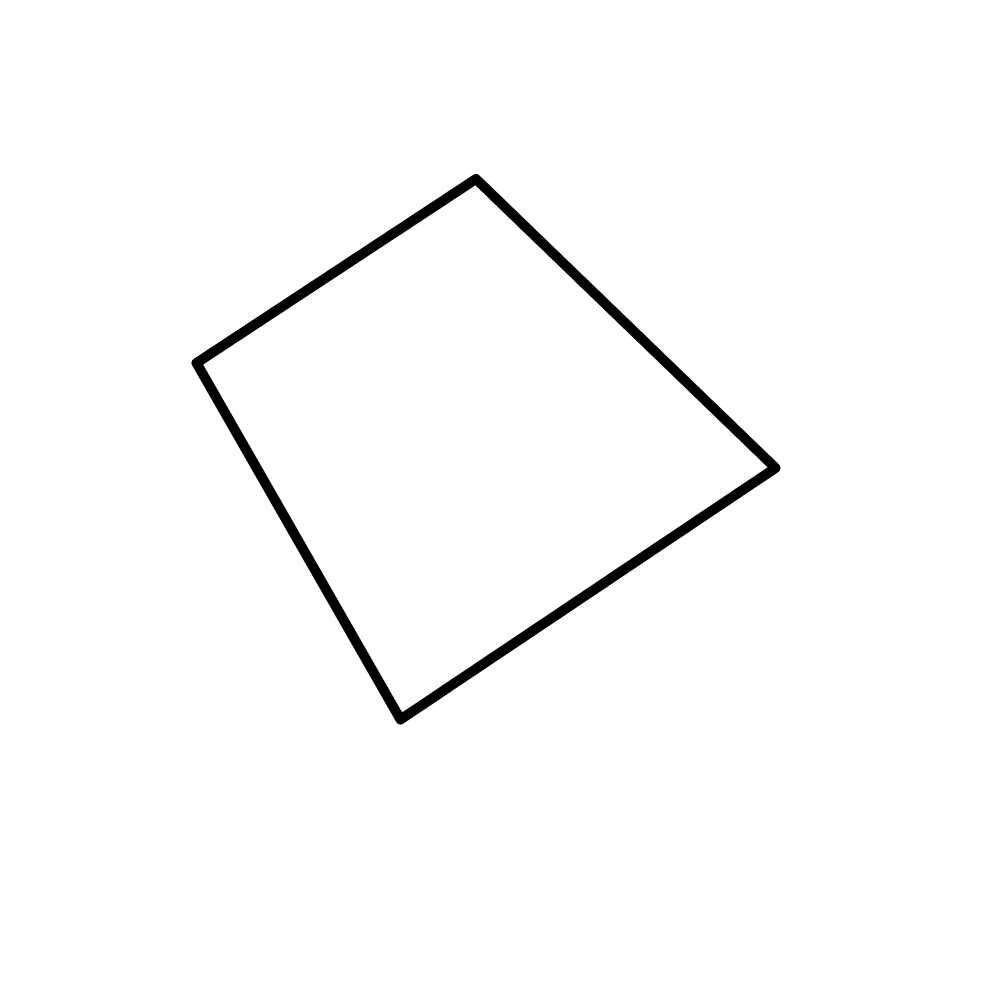
\includegraphics[width=.8\linewidth]{grundlagen/model/polygon.png}
    \caption{Polygon}
  \end{subfigure}%
  \begin{subfigure}{.5\textwidth}
    \centering
    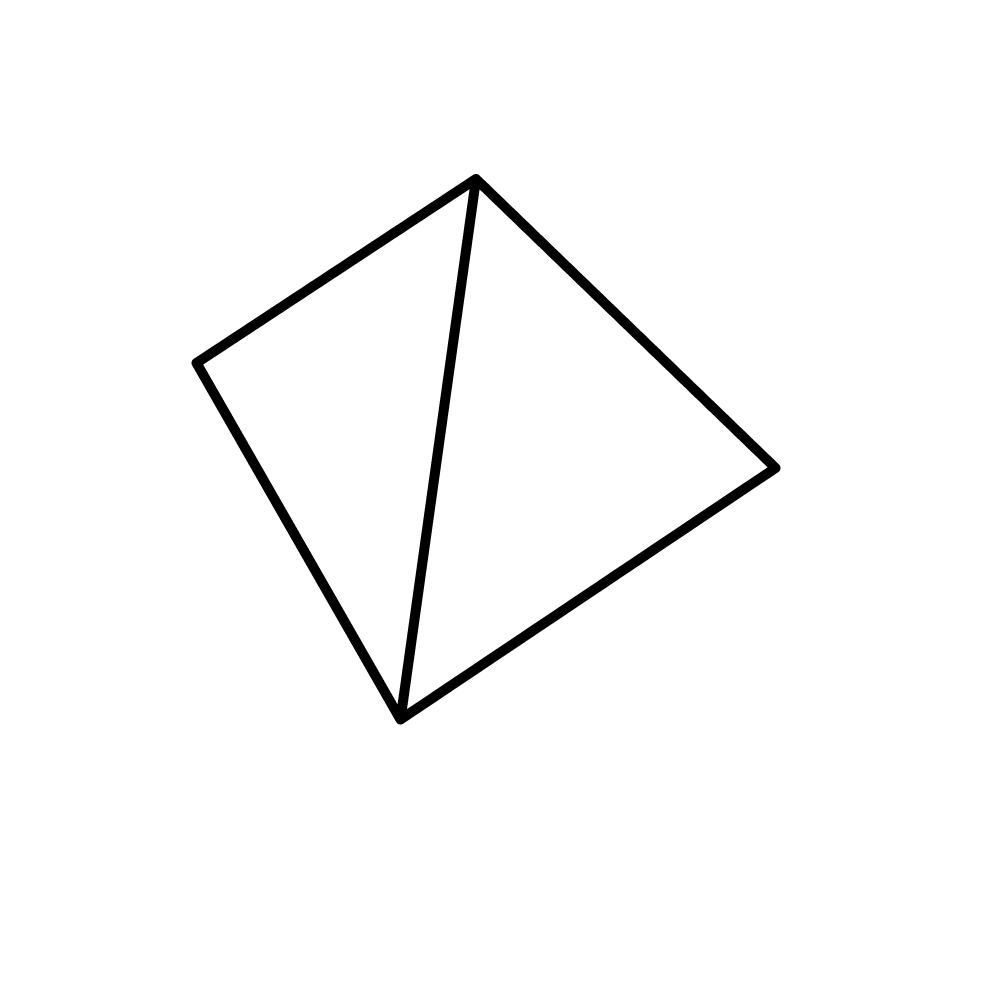
\includegraphics[width=.8\linewidth]{grundlagen/model/polygon-triangulation.png}
    \caption{Polygon als Sammlung von \e{Triangles}}
  \end{subfigure}
  \caption{Vereinfachung von Polygone als Sammlung von \e{Triangles}}
  \label{fig:modelSimpleTriangulation}
\end{figure}

\paragraph{Weitere Attribute}
Neben den geometrischen Attributen verfügt ein Modell über weitere Attribute, welche zum Beispiel die visuellen Aspekte definieren.

\subparagraph{Normals}

So wird für jeden \e{Vertex} ein \e{Normal} definiert. Ein \e{Normal} ist ein Vektor der im einfachsten Fall senkrecht zu den zwei an diesem \e{Vertex} verbundenen \e{Edges} verläuft. In diesem Fall ist sie identisch zur aus der Geometrie bekannten Normale. \e{Normals} werden häufig für das Berechnen von Reflexionen verwendet.
\e{Normals} werden auch für gewisse Performanzoptimierungen eingesetzt, dazu mehr in \autoref{chap:backfaceCulling}.

\subparagraph{Texturen}
Um die Oberfläche von Modellen zu definieren, wird häufig ein \e{Texture Mapping}, auch \e{UV-Mapping} genannt, durchgeführt. Bei diesem Verfahren wird definiert wie eine 2D-Grafik auf ein 3D-Modell abzubilden ist. Dafür wird für jeden \e{Vertex} zwei Koordinaten, $u$ und $v$, definiert. Diese Koordinaten definieren die Position in der 2D-Grafik. In der Praxis finden weitere Methoden Anwendung, auf diese wird hier im Sinne der Übersichtlichkeit nicht weiter eingegangen.

\paragraph{Abgrenzung}
Für diese Arbeit sind nur polygonale Modelle relevant.
Alternativen wie zum Beispiel \e{Point Clouds}, welche das Resultat von 3D-Scans sind, werden nicht weiter erläutert, da sie selten im Web eingesetzt werden. Auch andere Methoden wie \e{NURBS}, welche Modelle mithilfe von mathematisch definierten Flächen modelliert, werden deshalb aussen vor gelassen.

\paragraph{Formate}
Um ein 3D-Modell in einer Anwendung zu verwenden, muss ein entsprechendes Format verwendet werden. Hierfür steht eine Vielzahl von Optionen zur Auswahl. Aufgrund der Menge wird hier jedoch nur oberflächlich auf die bekanntesten Formate eingegangen.

\subparagraph{OBJ}
\e{Wavefront OBJ} ist ein offenes Dateiformat das von \e{Wavefront Technologies} 1989 entwickelt wurde. Das Format ist jedoch speichertechnisch ineffizient und verfügt zudem nur über einen limitierten Funktionsumfang. Des Weiteren gibt es keine zentrale Instanz, welche eine Spezifikation liefert und Informationen sind deshalb schwerer zu finden. \cite{objSpec}

\subparagraph{FBX}
\e{FBX} ist ein proprietäres Format, welches von Autodesk verwaltet wird. Das Verwenden von \e{FBX} Daten ist jedoch offiziell nur mit einer \e{C++ FBX \gls{SDK}} möglich, welche für das Web nicht geeignet ist. Aufgrund der proprietären Natur gibt es keine Bestrebungen das Format offener zu gestalten.

\subparagraph{glTF}
Seit 2015 gibt es ein offenes, modernes sowie auf optimale Speichernutzung fokussiertes Format: \e{glTF}. Dieses Format wird von der \e{Khronos Group} entwickelt \cite{gltf1Spec}. In dieser Arbeit wird es als Austauschformat verwendet, deshalb wird im folgenden genauer auf das Format eingegangen.

Die meisten 3D-Grafikprogramme wie Blender (.blend) verwenden ihre eigenen Dateiformate. Diese Dateiformate sind jedoch für den Einsatz in einer Applikation ungeeignet, da sie insbesondere nicht für die Laufzeitumgebung optimiert sind. Deswegen brauchte es für jedes Eingangsformat für jedes Ausgangsformat einen Konverter, wie in Abbildung \ref{fig:contentPipelineWithoutGltf} ersichtlich.

\begin{figure}[H]
  \centering
  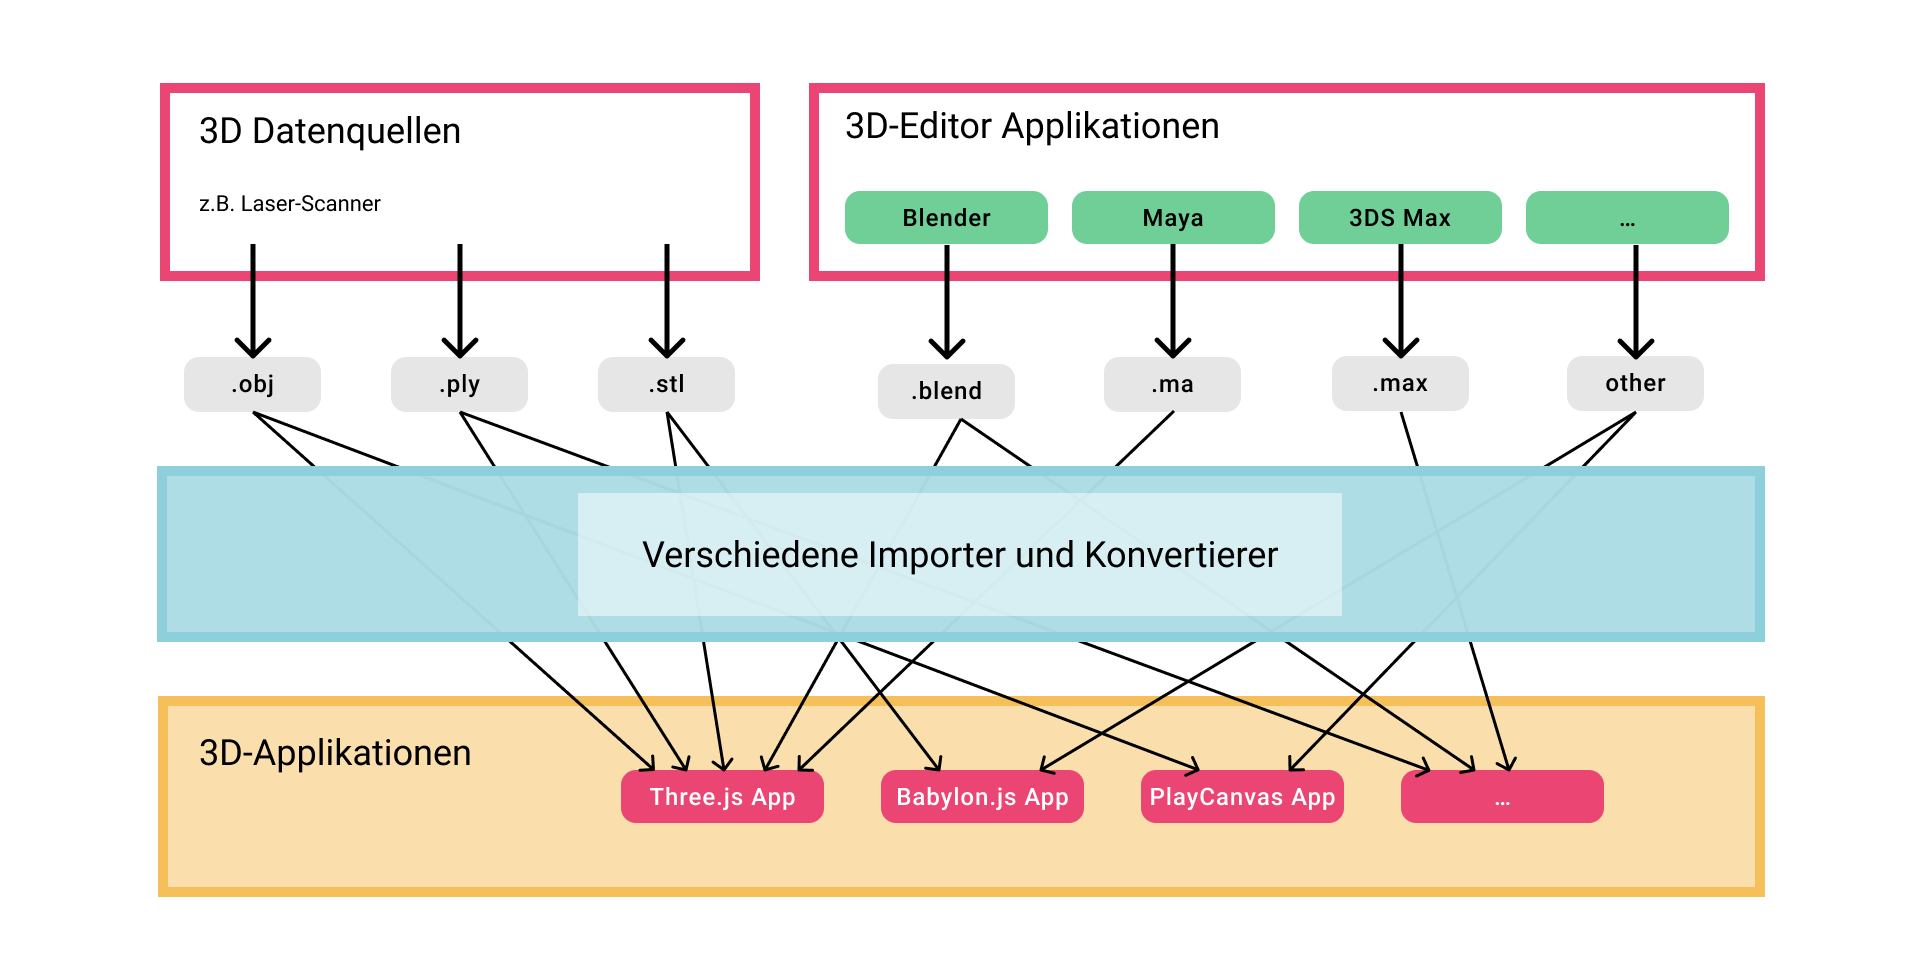
\includegraphics[width=1\columnwidth]{grundlagen/gltf/contentPipeline.png}
  \caption{Konvertierungspipeline ohne \e{glTF} \cite{gltfTutorialIntro}}
  \label{fig:contentPipelineWithoutGltf}
\end{figure}

Durch die immer grösser werdende Nachfrage nach 3D-Applikationen wurde ein Format benötigt, dass zum einen applikationsunabhängig verwendet und zum anderen performant im Web eingesetzt werden kann.
Durch diese Abstraktion kann eine Vielzahl Konverter vermieden werden und nur wenige, sehr spezifische Dateiformate benötigen noch einen einzigen Konverter. Diese neue Pipeline ist in Abbildung \ref{fig:contentPipelineWithGltf} dargestellt. \cite{gltfTutorialIntro}
\begin{figure}[H]
  \centering
  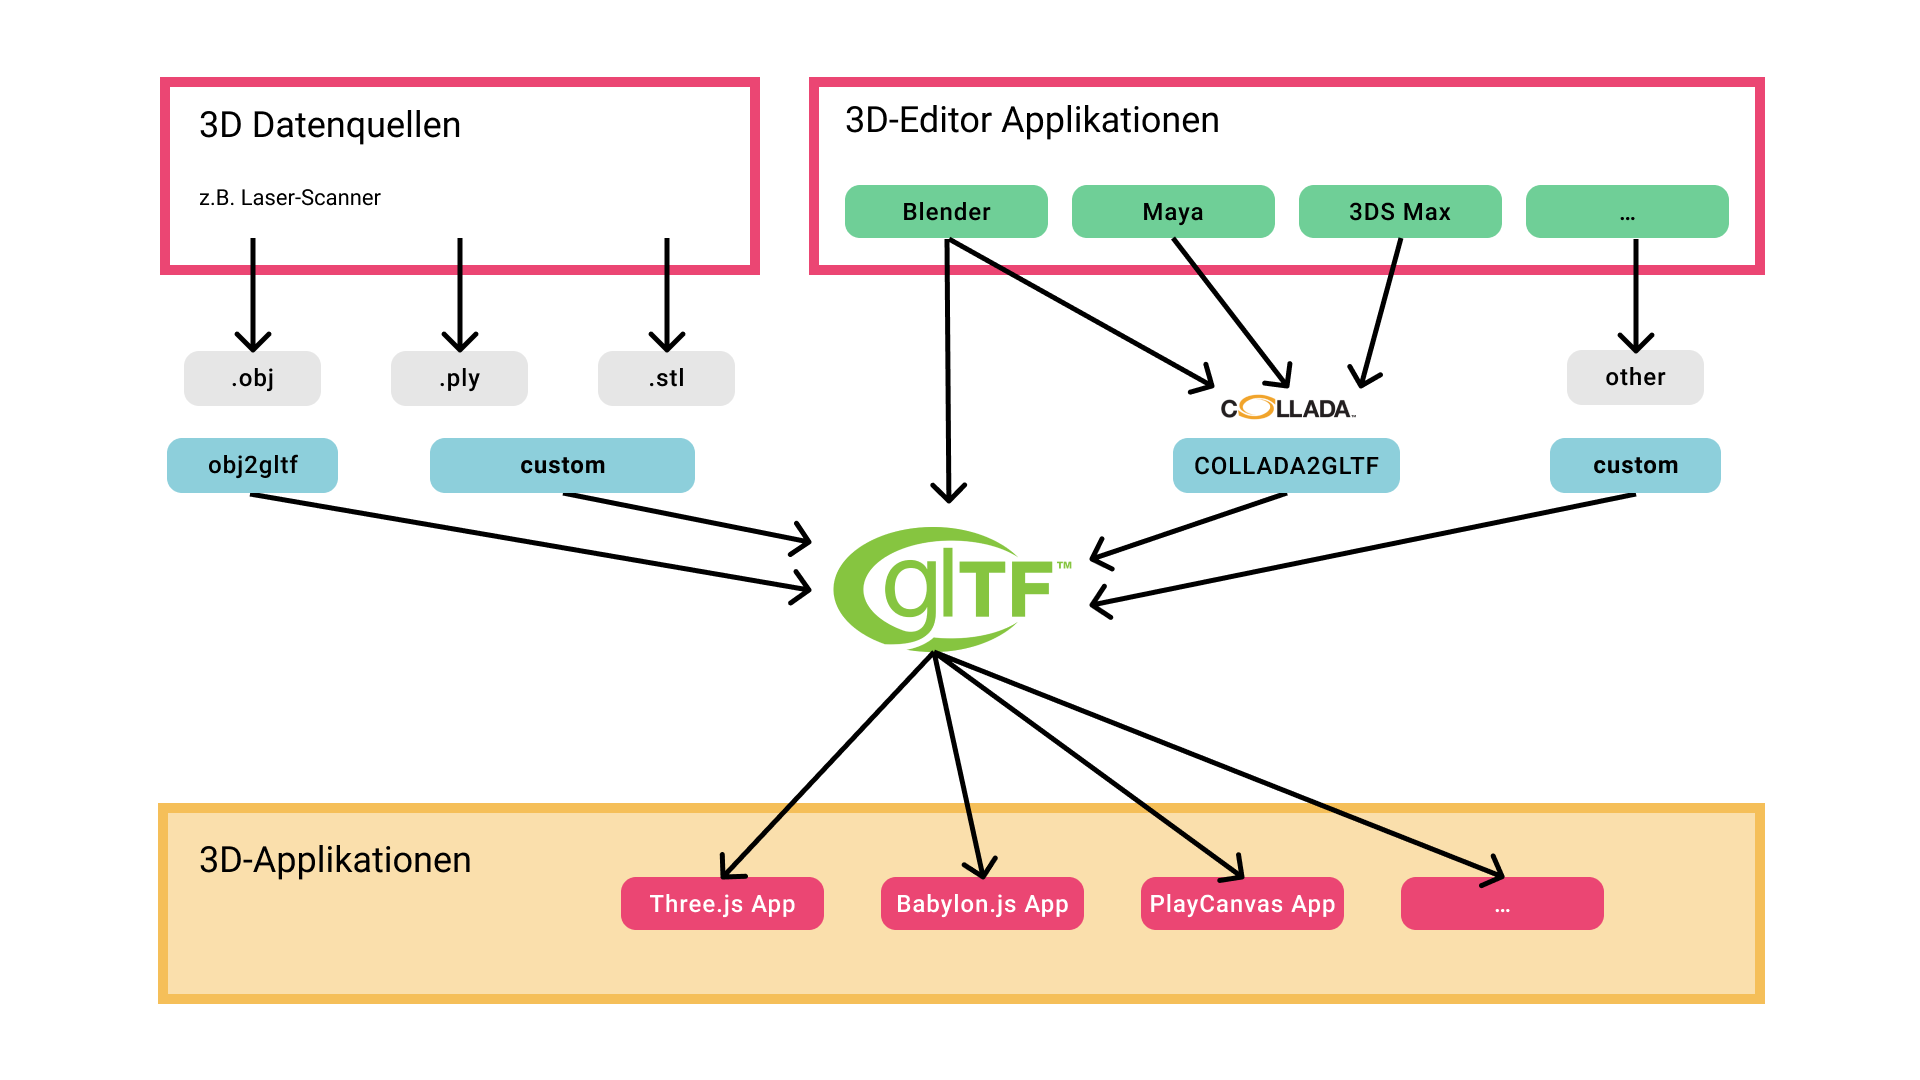
\includegraphics[width=1\columnwidth]{grundlagen/gltf/contentPipelineWithGltf.png}
  \caption{Konvertierungspipeline mit \e{glTF} \cite{gltfTutorialIntro}}
  \label{fig:contentPipelineWithGltf}
\end{figure}

Die Basisstruktur von \e{glTF} basiert auf \fgls{JSON}{JavaScript Object Notation, Austauschformat, welches häufig in der Web-Entwicklung eingesetzt wird}. Darin ist die komplette Szenerie des Modells beschrieben und in Abbildung \ref{fig:gltfDatastructure} aufgezeigt \cite{gltfTutorialStructure}.
\begin{figure}[H]
  \centering
  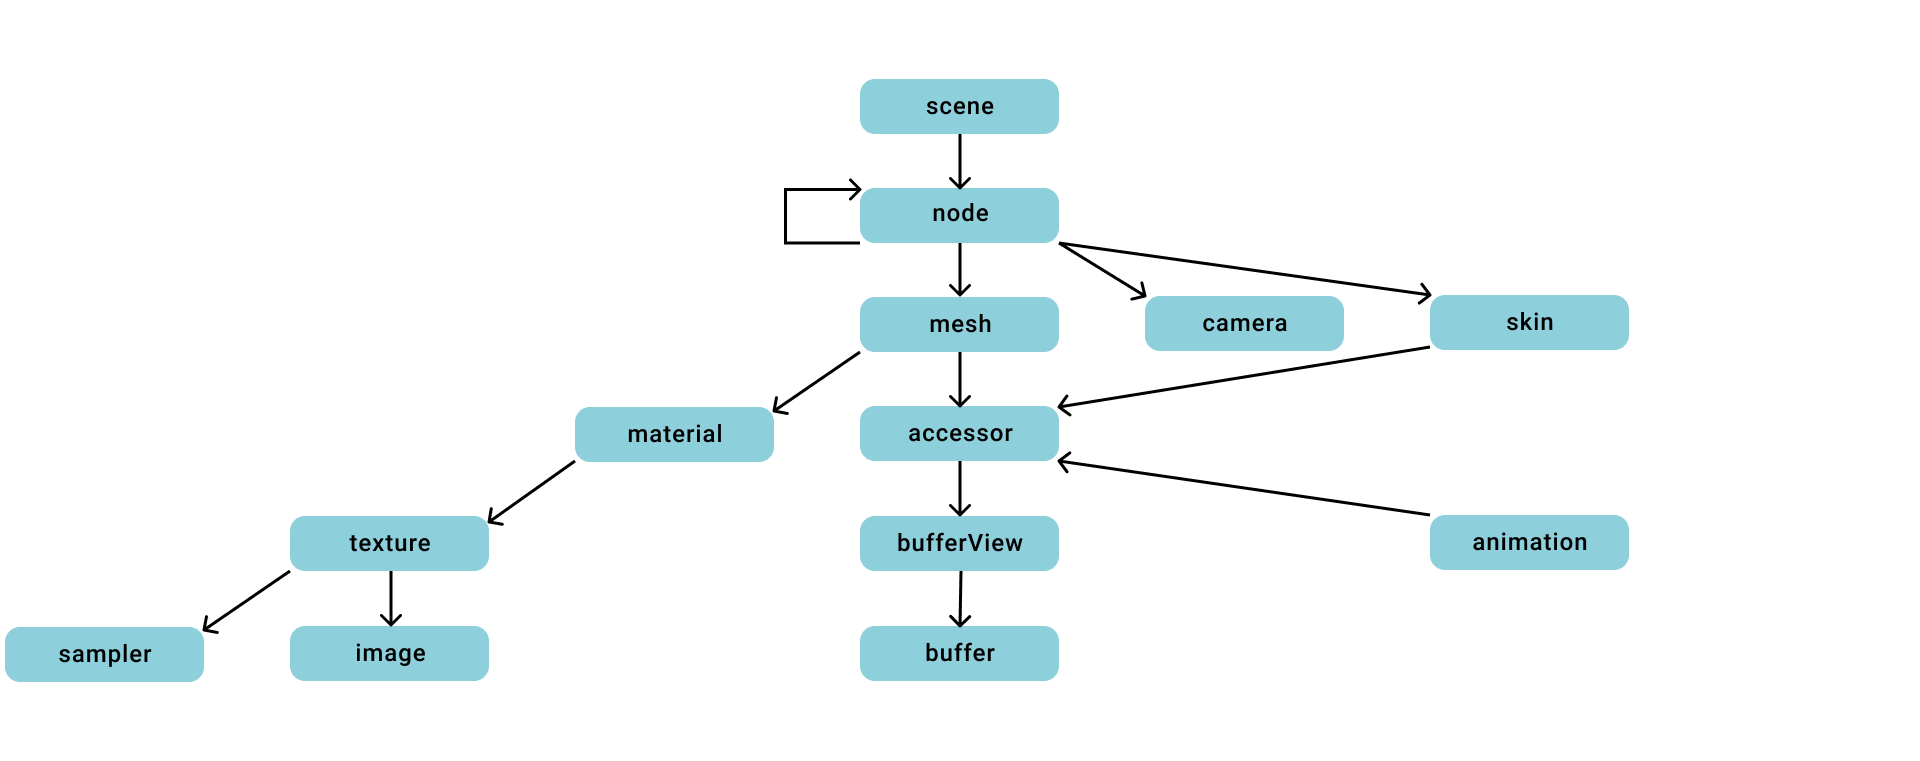
\includegraphics[width=1\columnwidth]{grundlagen/gltf/gltfJsonStructure.png}
  \caption{\e{glTF} Datenstruktur \cite{gltfTutorialStructure}}
  \label{fig:gltfDatastructure}
\end{figure}

Die wichtigsten Elemente dieser Struktur kurz erläutert:
\begin{itemize}
  \item \textbf{Scene}: Einstiegspunkt der Szenerie und verweist auf alle Top-Level \e{nodes}.
  \item \textbf{Node}: Kann eine Transformation (Rotation, Translation oder Skalierung) beinhalten oder eine Kamera, \e{Skin}, Animation, ein \e{Mesh} oder \e{Childnodes} referenzieren.
  \item  \textbf{Mesh}: Beschreibt ein geometrisches Objekt und verweist auf \e{accessor}, welcher die effektiven geometrischen Daten beinhaltet und auf \e{material}, das beschreibt, wie das Objekt beim Rendern aussehen soll.
  \item \textbf{Accessor}: Verweis auf die \e{BufferView}, welche die effektiven Eigenschaften für \e{meshes}, \e{skins} und \e{animations} kompakt beinhaltet.
  \item \textbf{BufferView}: Definiert eine Ansicht (Länge, Ort, Typ) auf einen \e{Buffer}.
  \item \textbf{Buffer}: Verweist auf einen Block von Binärdaten, welchen die effektiven Daten des 3D-Modells beinhaltet.
  \item \textbf{Material}: Definiert die visuellen Attribute eines \e{Mesh}.
  \item \textbf{Texture}: Definiert wie ein \e{Image} auf ein \e{Material} projiziert wird. Ein \e{Sampler} definiert wie das Bild platziert werden soll.
  \item Weitere Elemente, welche im Rahmen dieser Arbeit nicht relevant sind und nicht im Detail betrachtet werden, sind: \e{camera}, \e{skin} und \e{animation}.
\end{itemize}

\section{Transformation von Modellen}

Um ein Modell vereinfachen zu können, muss es verändert werden.
Diese Veränderungen können in Operationen vereinfacht erläutert werden.

Im Folgenden werden Transformationen mithilfe einer 2D-Visualisierung erläutert. Das Modell kann jedoch ebenfalls im dreidimensionalen Raum sein – die Funktionsweise bleibt identisch.

Für die folgenden Beispiele wird jeweils das Modell aus Abbildung \ref{fig:transformationOriginal} verwendet.

\begin{figure}[H]
  \centering
  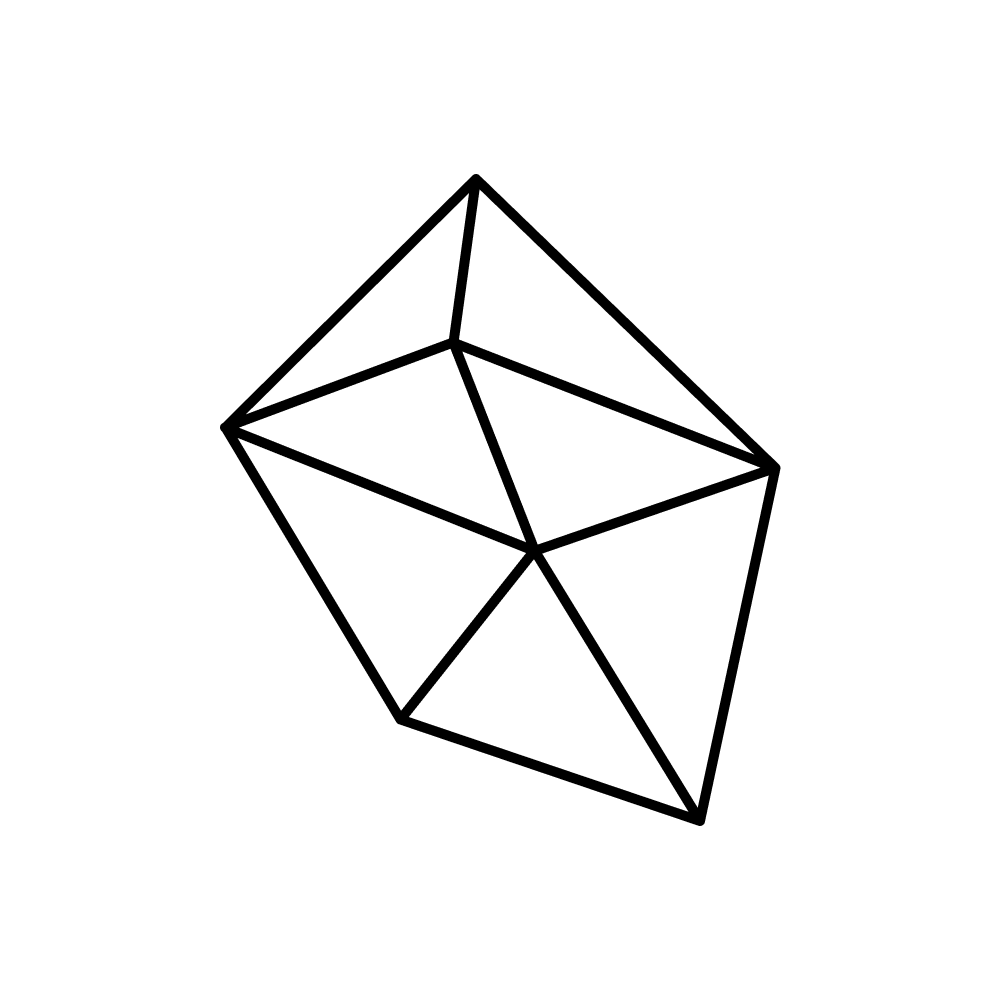
\includegraphics[width=0.3\columnwidth]{grundlagen/transformationen/original.png}
  \caption{Modell Basis}
  \label{fig:transformationOriginal}
\end{figure}

\paragraph{Edge Collapse}
Hierbei werden zwei nebeneinanderliegende \e{Vertices} kombiniert. Durch diese Operation kann ein \e{Vertex} entfernt werden. In Abbildung \ref{fig:transformationEdgeCollapse} kann die Anzahl \e{Triangles} um zwei verringert werden. Beim \e{Edge Collapse} wird ein neuer \e{Vertex} definiert und zwei bestehende entfernt. Die Anzahl entfernter \e{Triangles} ist abhängig von der Situation. Unter Umständen kann so auch nur ein einzelner \e{Triangle} entfernt werden.
Die Umkehrfunktion nennt man \e{Vertex} Split.

\begin{figure}[H]
  \centering
  \begin{subfigure}{.5\textwidth}
    \centering
    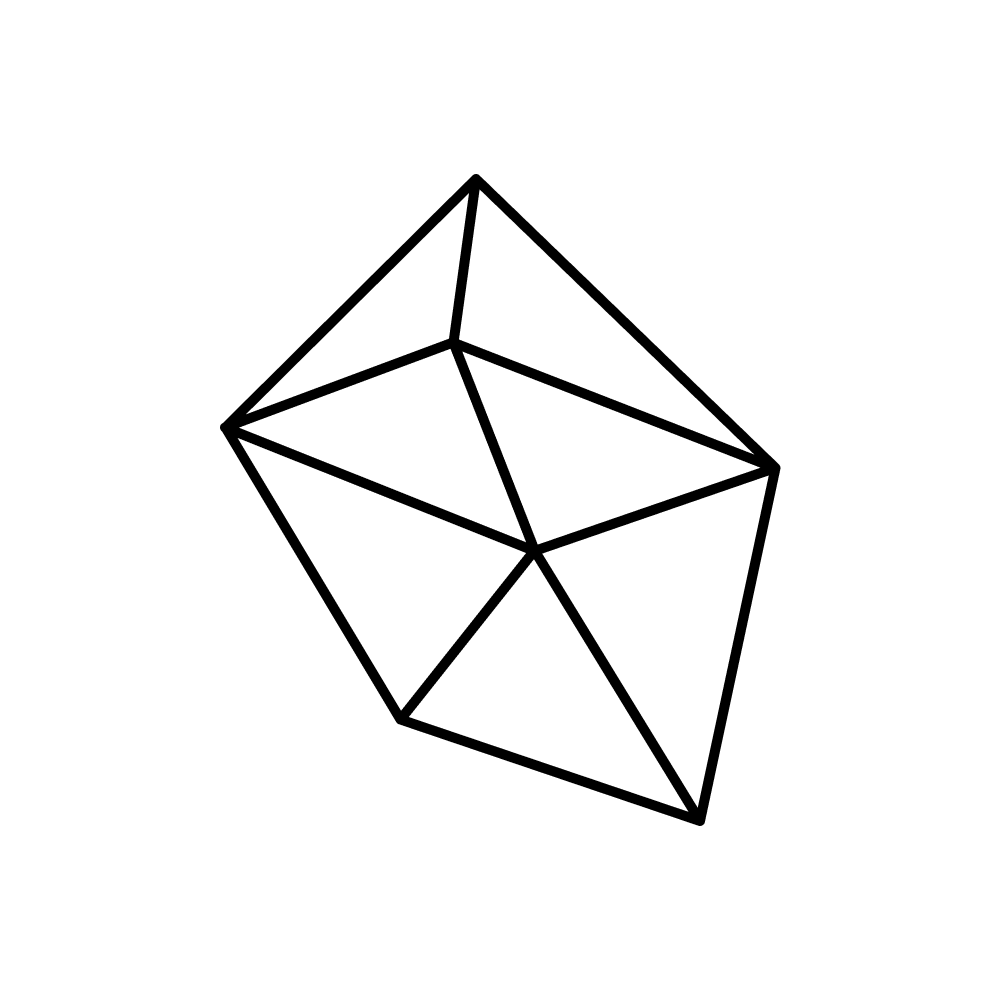
\includegraphics[width=.7\linewidth]{grundlagen/transformationen/original.png}
    \caption{Modell Ausgangslage}
  \end{subfigure}%
  \begin{subfigure}{.5\textwidth}
    \centering
    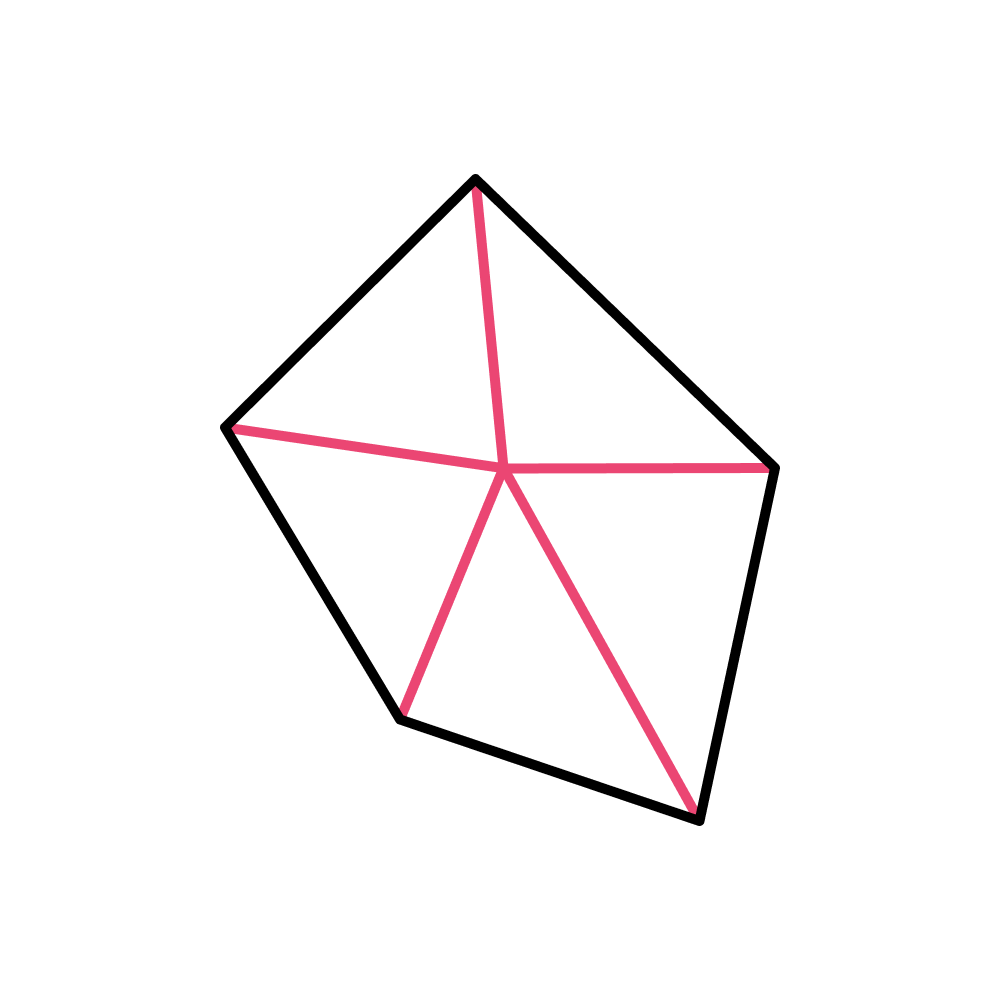
\includegraphics[width=.7\linewidth]{grundlagen/transformationen/edge-collapse.png}
    \caption{\e{Edge Collapse}}
  \end{subfigure}
  \caption{Transformation mittels \e{Edge Collapse}}
  \label{fig:transformationEdgeCollapse}
\end{figure}

\paragraph{Halfedge Collapse}
Hierbei wird ein Vertex direkt entfernt und alle \e{Edges} auf einen danebenliegenden Vertex zusammengelegt. Bei dieser Operation muss kein neuer Vertex definiert werden, sondern ein bereits bestehender Vertex kann wiederverwendet werden. Wie in Abbildung \ref{fig:transformationHalfedgeCollapse} ersichtlich, können auch in diesem Fall zwei \e{Triangles} entfernt werden.

\begin{figure}[H]
  \centering
  \begin{subfigure}{.5\textwidth}
    \centering
    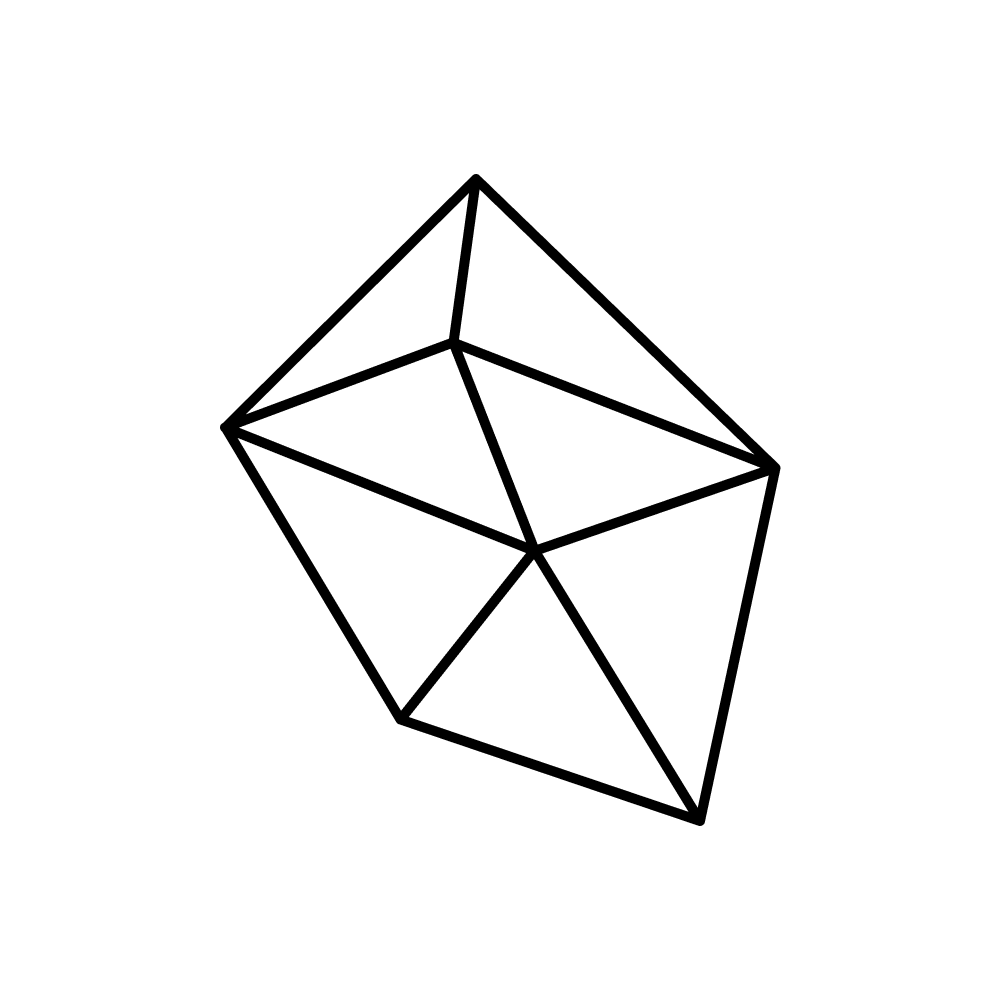
\includegraphics[width=.7\linewidth]{grundlagen/transformationen/original.png}
    \caption{Modell Ausgangslage}
  \end{subfigure}%
  \begin{subfigure}{.5\textwidth}
    \centering
    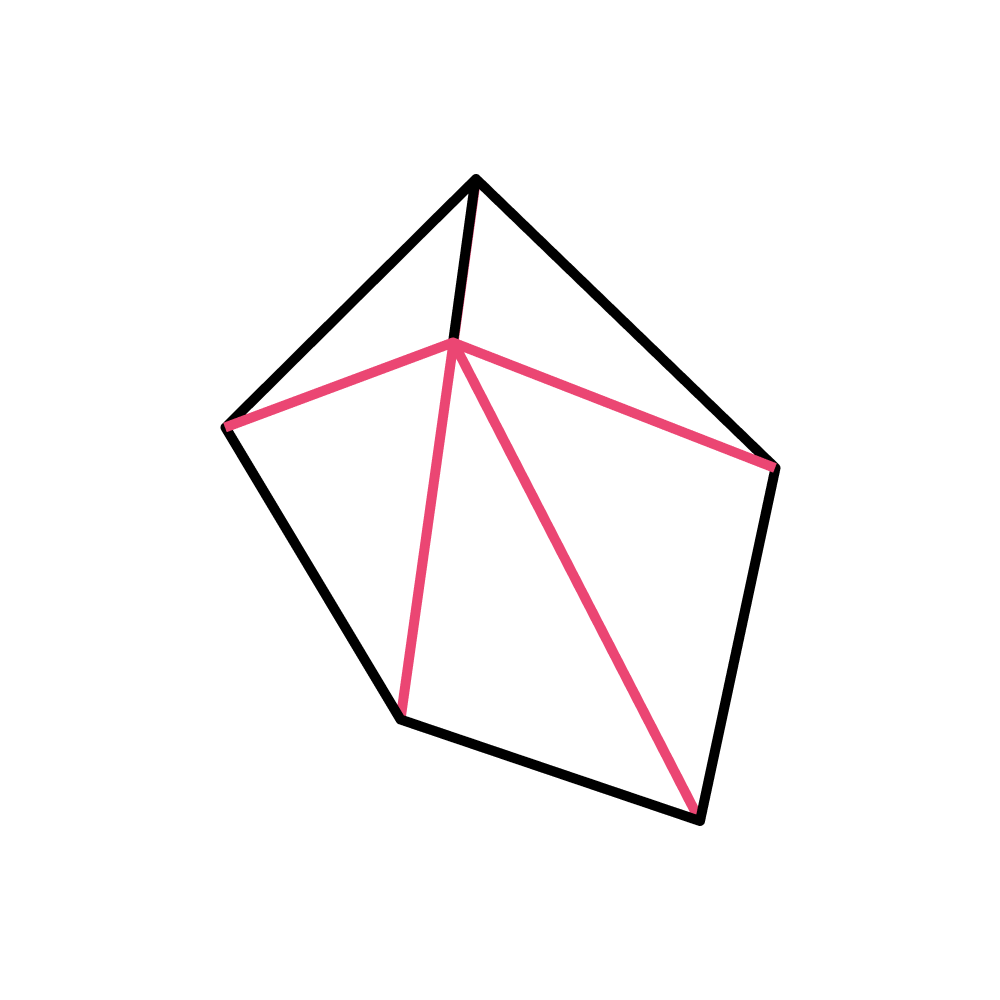
\includegraphics[width=.7\linewidth]{grundlagen/transformationen/half-edge-collapse.png}
    \caption{\e{Halfedge Collapse}}
  \end{subfigure}
  \caption{Transformation mittels \e{Halfedge Collapse}}
  \label{fig:transformationHalfedgeCollapse}
\end{figure}

\paragraph{Vertex Removal}
Hierbei wird ein Vertex entfernt und das Resultat neu trianguliert. Triangulation ist ein Verfahren, um ein Polygon in \e{Triangles} aufzuteilen.
In Abbildung \ref{fig:transformationVertexRemovalOriginal} wird der zentrale Vertex entfernt. Anschliessend werden alle \e{Triangles} an diesem Punkt entfernt. Das dabei entstehende Loch wird neu mit \e{Triangles} gefüllt. Eine mögliche Triangulation des Polygons ist in Abbildung \ref{fig:transformationVertexRemovalFinal} ersichtlich.

\begin{figure}[H]
  \centering
  \begin{subfigure}{.5\textwidth}
    \centering
    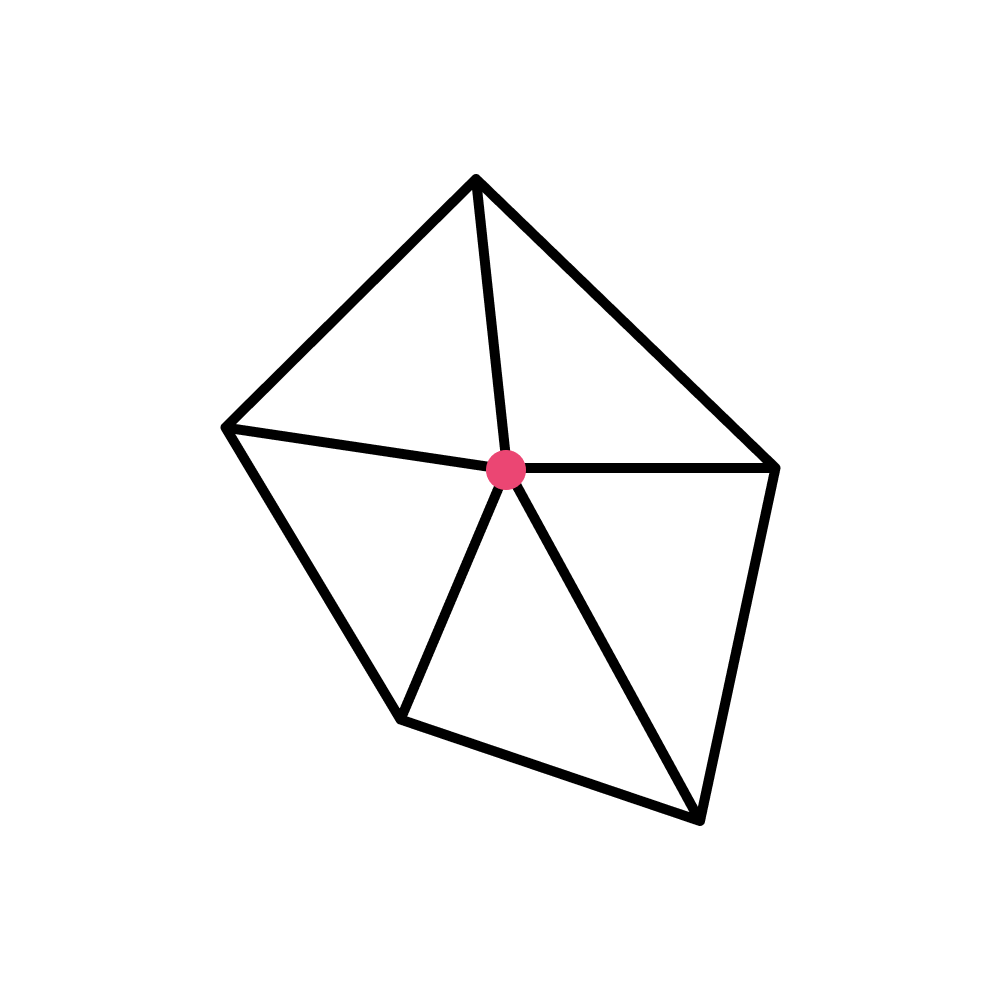
\includegraphics[width=.7\linewidth]{grundlagen/transformationen/vertex-removal-original.png}
    \caption{Modell Ausgangslage}
    \label{fig:transformationVertexRemovalOriginal}
  \end{subfigure}%
  \begin{subfigure}{.5\textwidth}
    \centering
    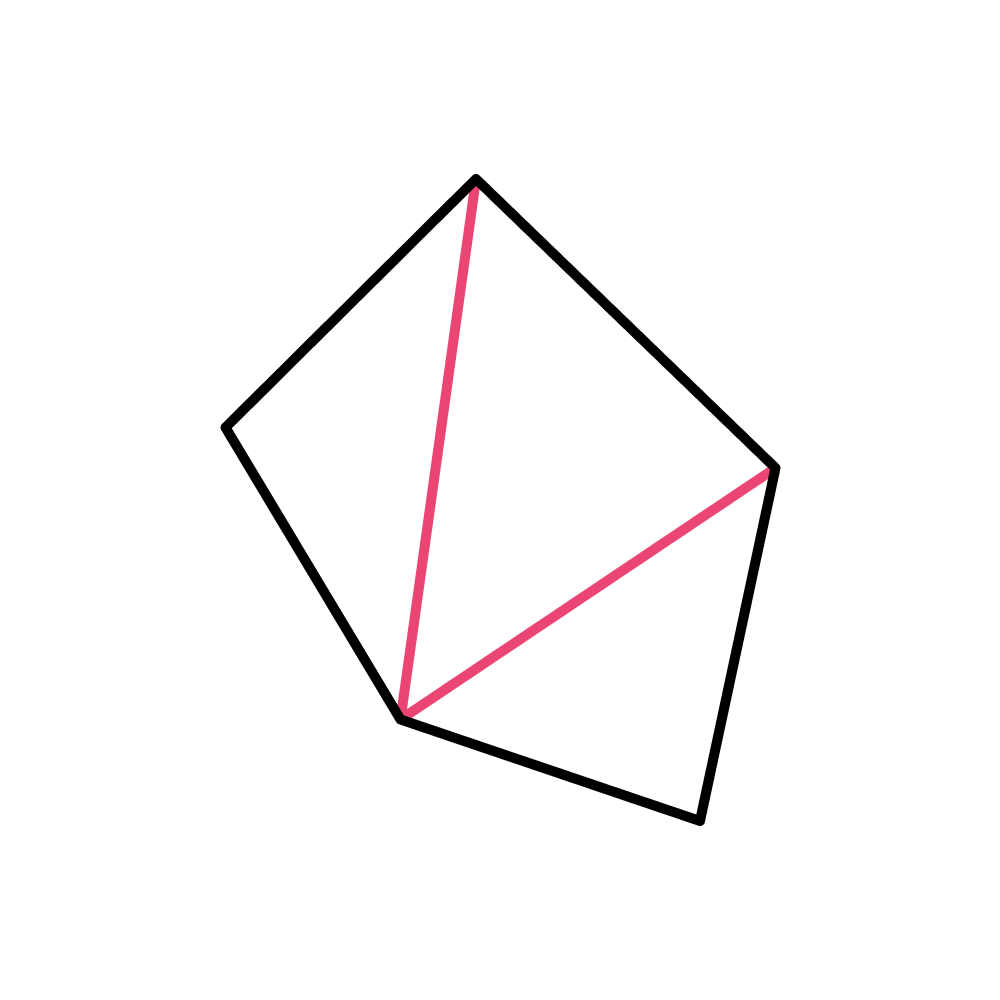
\includegraphics[width=.7\linewidth]{grundlagen/transformationen/vertex-removal-final.png}
    \caption{Vertex Removal}
    \label{fig:transformationVertexRemovalFinal}
  \end{subfigure}
  \caption{Transformation mittels Vertex Removal}
  \label{fig:transformationVertexRemoval}
\end{figure}

\section{Grafikpipeline}

Die Grafikpipeline ist zuständig um eine definierte Szene auf einem Ausgabegerät zu visualisieren. Die Schritte werden im folgenden Abschnitt nur oberflächlich erläutert, um ein grobes Verständnis zu vermitteln. Es wird dabei ein simples 3D-Modell auf einem 2D-Display, wie zum Beispiel einem Monitor, visualisiert. Die Schritte sind in Abbildung \ref{fig:renderingPipelineOverview} aufgezeigt. Der Prozess wird idealerweise 60 Mal pro Sekunde wiederholt. Dies findet in der sogenannten \e{Render Loop} statt.

\begin{figure}[H]
  \centering
  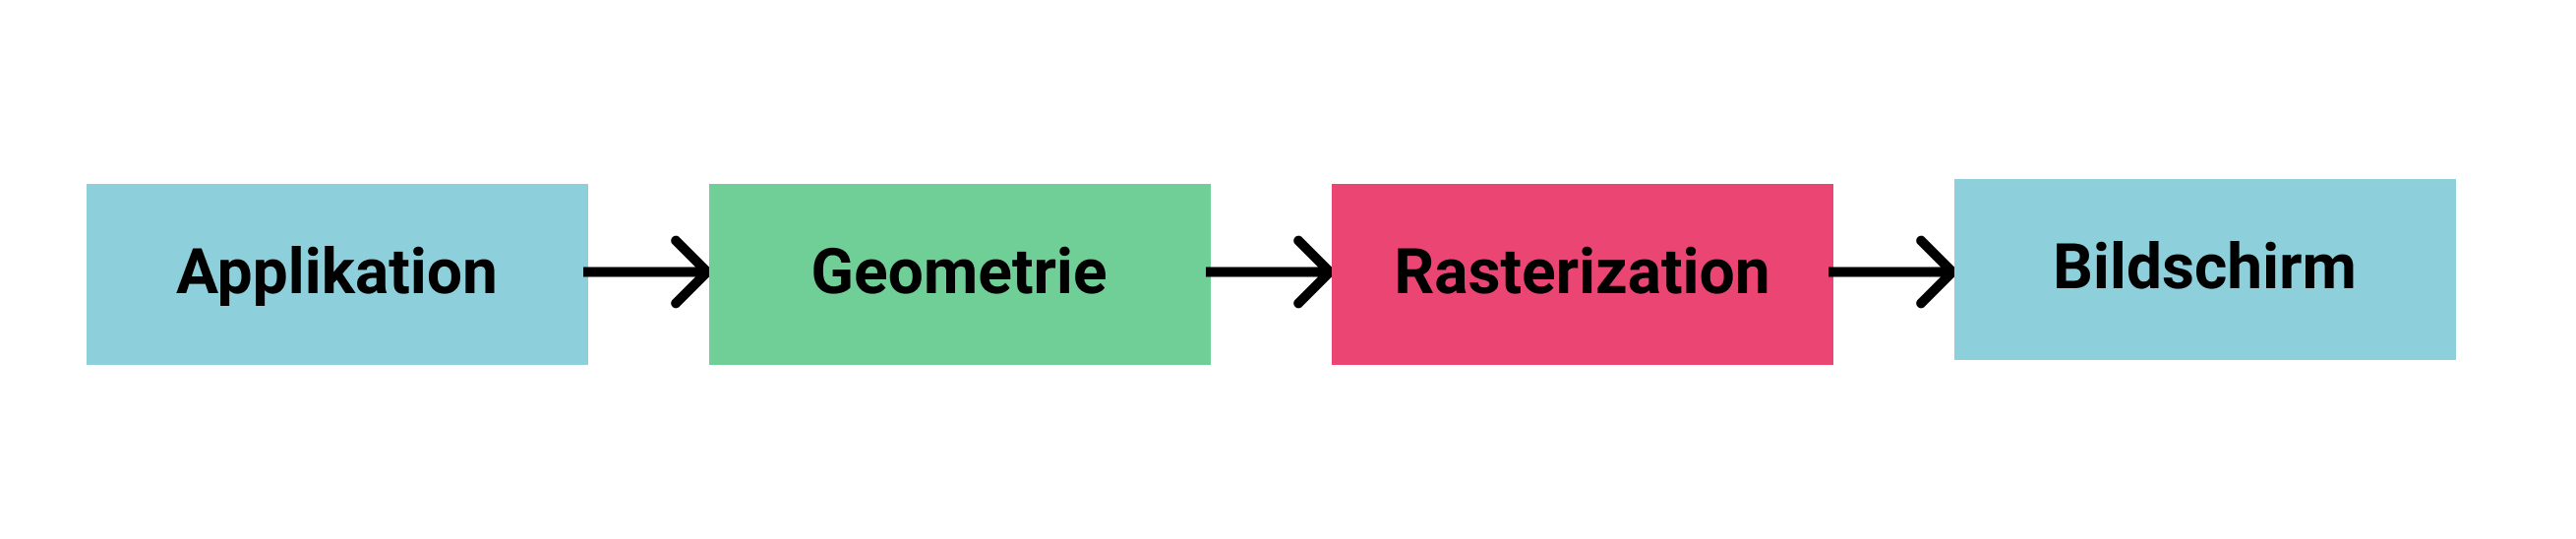
\includegraphics[width=0.8\columnwidth]{grundlagen/pipeline/graphics-pipeline.png}
  \caption{Schritte einer Realtime Rendering Pipeline}
  \label{fig:renderingPipelineOverview}
\end{figure}

\paragraph{Applikation}
Im ersten Schritt wird die Szenerie aufbereitet, Modelle in den Arbeitsspeicher geladen und Positionen und Rotationen der Modelle definiert. Diese Schritte werden auf der \e{\gls{CPU}} durchgeführt. Ein Beispiel für das Aufsetzen eines einfachen \e{Triangles} bestehend aus drei \e{Vertices} ist in Abbildung \ref{fig:geometryDefinition} ersichtlich. Das \e{Triangle} wird anschliessend mithilfe dreier \e{Indices} definiert. Diese \e{Indices} verweisen auf die entsprechenden \e{Vertices}. So entspricht der Eintrag $0$ dem \e{Vertex} an der Position $V_0$. Wobei $V_0$ definiert ist als:

$$
V_0 = \begin{bmatrix}
  -1 \\
  1 \\
  0
\end{bmatrix}
$$

\begin{figure}[H]
\begin{lstlisting}[style=JavaScript]
const vertices = new Float32Array([
  -1, 1, 0, // vertex 0
  -1, -1, 0, // vertex 1
  1, -1, 0 // vertex 2
]);

const indices = new Uint16Array(
  [0, 1, 2] // triangle 0
);
\end{lstlisting}
\caption{Definition eines Triangles}
\label{fig:geometryDefinition}
\end{figure}

Anschliessend werden die Daten in einem \e{Draw Call} an die \e{\gls{GPU}} gesendet. Ein \e{Draw Call} wird pro Material pro \e{Mesh} benötigt. Es ist besser, weniger, dafür umfangreiche \e{Draw Calls} abzusetzen, als viele Kleinere. Dies kommt daher, dass die \e{\gls{GPU}} grosse Datenmengen parallel prozessieren kann und sich die Unterbrechung durch einzelne Aufrufe negativer auswirkt.

\paragraph{Vertexshader}
Der erste Schritt ist der sogenannte Vertexshader. Auftrag des Vertexshaders ist es, die \e{Vertices} zu transformieren. Die Modelle werden ausgerichtet, die Beleuchtung bestimmt und die 2D-Projektion vorgenommen. Ein Beispiel für einen simplen Vertexhsader ist in Abbildung \ref{fig:vertexShader} ersichtlich. Der Code, welcher in \fgls{GLSL}{OpenGL Shading Language, C-basierte Programmiersprache für das Programmieren von \e{\gls{GPU}}-Prozessen} geschrieben ist, wird für jeden \e{Vertex} ausgeführt. Der aktuelle \e{Vertex} ist dabei in der Variable \e{coordinates} abgespeichert. \e{gl\_Position} ist eine spezielle Variable, welche von \e{GLSL} zur Verfügung gestellt wird und den Endpunkt beinhalten soll. Das gegebene Beispiel ist trivial, in der Praxis werden hier häufig die Matrixtransformationen unter anderem für die Kameraperspektive durchgeführt.

\begin{figure}[H]
\begin{lstlisting}[style=glsl]
attribute vec3 coordinates;

void main(void) {
  gl_Position = vec4(coordinates, 1.0);
}
\end{lstlisting}
\caption{Vertexshader für die Definition eines Punktes}
\label{fig:vertexShader}
\end{figure}

\paragraph{Fragmentshader}
Durch die Rasterisierung werden kontinuierliche Objekte zu diskreten Fragmenten verarbeitet. Ein Fragment entspricht grundsätzlich einem Pixel. Der Fragmentshader generiert die Farbdefinitionen für die einzelnen diskreten Fragmente. Dies können einfache Farbwerte sein, es ist jedoch auch möglich Texturen und dergleichen auf Fragmente abzubilden. Ein einfaches Beispiel für einen Fragmentshader ist in Abbildung \ref{fig:fragmentShader} ersichtlich. Bei \e{gl\_FragColor} handelt es sich wiederum um eine Variable von \e{GLSL}. Der zugewiesene Wert entspricht der Farbe des Pixels. In diesem Fall ist die Farbe Schwarz. Das Format entspricht rgba: rot, grün, blau, alpha (Transparenz).

\begin{figure}[H]
\begin{lstlisting}[style=glsl]
void main(void) {
  gl_FragColor = vec4(0.0, 0.0, 0.0, 1.0);
}
\end{lstlisting}
\caption{Fragmentshader für das definieren von Farbwerten}
\label{fig:fragmentShader}
\end{figure}


\paragraph{Bildschirm}
Am Schluss wird für jedes vom Fragmentshader generierte Fragment ein Sichtbarkeitstest durchgeführt. So werden nur die Fragmente, welche von keinem anderen Fragment überdeckt werden, angezeigt. Das generierte Bild wird im Anschluss skaliert und auf dem Bildschirm dargestellt.


\section{Performanzoptimierung}
Visualisierungen können zu komplex werden, um jederzeit performant und interaktiv gerendert zu werden.
Insbesondere wenn viele Objekte gleichzeitig sichtbar sind, lohnt es sich Performanzoptimierungen durchzuführen.
Im Idealfall geschieht dies jedoch, ohne dass der Anwender dies bemerkt.

In diesem Abschnitt werden mögliche Ansätze erklärt, welche helfen sollen, die Render-Performanz zu erhöhen. Diese Arbeit konzentriert sich jedoch auf den Ansatz von Level of Detail; die anderen Ansätze werden nur kurz erläutert. Auf Level of Detail wird in \autoref{chap:lodIntroduction} detailliert eingegangen.

\paragraph{Frustum culling}
Ein Frustum ist eine geometrische Form, die einer Pyramide ähnelt, welcher die Spitze abgeschnitten wurde.
Das Kamera-Frustum bezeichnet den Raum, welcher von der Kamera aufgezeichnet wird. Dieser Bereich startet eine gewisse Distanz von der Kamera entfernt und endet weit hinten wieder, da nicht bis in die Unendlichkeit Objekte sichtbar sind.
Wie in Abbildung \ref{fig:CameraFrustum} zusehen ist, beginnt das Kamera-Frustum in der Nähe der Kamera und dehnt sich ein wenig aus bis es gegen Ende des Spektrums beschränkt wird.
Polygone, welche nicht im Kamera Frustum enthalten sind, werden bei dieser Methode, wie in Abbildung \ref{fig:FrustumCulling} gezeigt, nicht weiter prozessiert.
Dies reduziert die Anzahl Polygone drastisch.

\begin{figure}[H]
  \centering
  \begin{subfigure}{.5\textwidth}
    \centering
    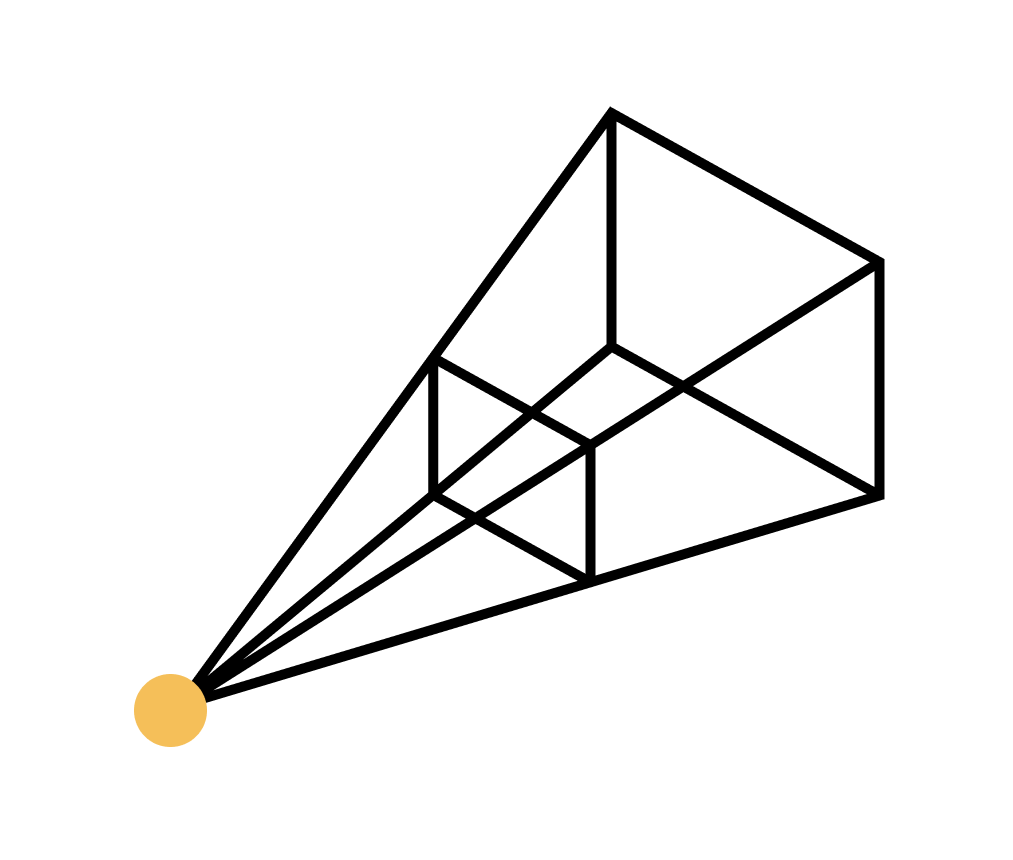
\includegraphics[width=0.5\columnwidth]{grundlagen/Camera-Frustum.png}
    \caption{Kamera Frustum}
    \label{fig:CameraFrustum}
  \end{subfigure}%
  \begin{subfigure}{.5\textwidth}
    \centering
    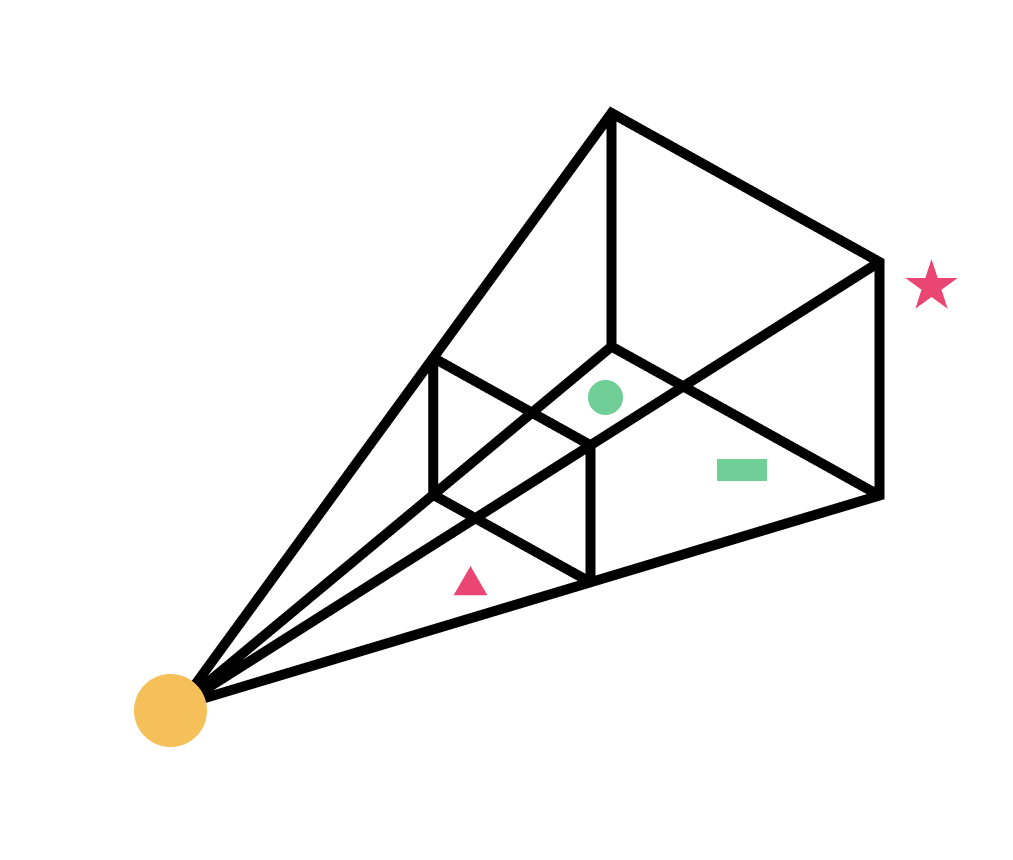
\includegraphics[width=0.5\columnwidth]{grundlagen/Frustum-Culling.png}
    \caption{Frustum culling visualisiert. Rote Elemente werden nicht prozessiert.}
    \label{fig:FrustumCulling}
  \end{subfigure}
  \caption{Frustum Culling}
\end{figure}

\paragraph{Occlusion culling}
Polygone bzw. Objekte, welche komplett von anderen Objekten überdeckt werden, werden bei dieser Variante nicht prozessiert.
Dieser Prozess analysiert die Szene mittels einer virtuellen Kamera und merkt sich potenziell nicht sichtbare Objekte. Diese Daten werden dann zur Laufzeit von der Kamera verwendet, um zu bestimmen, ob ein Objekt prozessiert werden soll, oder nicht.
Damit wird die Anzahl \e{Polygone}, welche gerendert werden müssen, reduziert.

\paragraph{Backface culling}
\label{chap:backfaceCulling}
Bei dieser Methode wird berechnet welche Polygone zur Kamera orientiert sind.
Alle Polygone, welche in die andere Richtung zeigen werden nicht gezeichnet.
Dies ist nicht immer gewünscht, für die meisten Anwendungen ist diese Optimierung jedoch aktiviert.
Als Grundlage für die Berechnung werden die \e{Normals} der \e{Vertices} verwendet.

\paragraph{Impostors}
Vergleichbar zu \e{LOD}-Artefakten sind sogenannte \e{Impostors}. Dabei wird ein \e{Quad} mit verschiedenen Texturen verwendet. Für jede mögliche Position des Modells wird eine Textur generiert. Das \e{Quad} wird in Richtung Kamera ausgerichtet und abhängig von der Rotation des Modells die geeignete Textur verwendet. Geometrisch kann ein Modell so auf ein absolutes Minimum reduziert werden. Schwierigkeiten dieser Methode sind Modelle, welche spezielle Materialien aufweisen. So ist zum Beispiel das Abbilden von Reflexionen, wie dies bei metallischen Oberflächen der Fall ist, eine Herausforderung \cite{usingImpostors}.

\paragraph{Weitere Ansätze}
Weitere Ansätze zur Optimierung der Performanz für sehr spezifische Anwendungsfälle werden kurz erwähnt, jedoch nicht weiter erörtert da sie für viele Anwendungen nicht praktikabel sind.

\subparagraph{Parallel rendering}
Auch bekannt unter \e{Distributed Rendering} ist der Einsatz von Techniken aus dem \e{Parallel Programming} in Visualisierungsanwendungen. So kann die Aufgabe auf verschiedene \e{\gls{GPU}}s verteilt parallel verarbeitet werden. Eine Problemstellung hierbei ist jedoch, dass das sinnvolle Aufteilen der Arbeit nicht trivial ist. So eignet sich dieser Ansatz jedoch gut für Anwendungen im Bereich von \e{Virtual Reality}, da dort zwei separate Bilder generiert werden müssen und somit leicht zu separieren sind \cite{parallelRenderingPhd}.

\subparagraph{Image-based rendering}
In gewissen Fällen kann das Modellieren übersprungen werden. So kann anhand von Bildmaterial eine 3D-Illusion erzeugt werden. Da 2D-Bilder aber keine Tiefeninformationen darstellen können im dreidimensionalen Raum, kann dies zu seltsamen Effekten führen, wenn sich die Kamera bewegt und kann deshalb nur in sehr spezifischen Anwendungsfällen eingesetzt werden. Die \e{Street View} Funktion von Google Maps ist ein bekanntes Tool, welches auf \e{Image-based rendering} setzt.
Beim Bewegen durch die virtuelle Welt in \e{Street View}, ist auffällig zu sehen, wie sich die Bilder austauschen \cite{imageBasedRendering}.

\section{Einführung Level of Detail}
\label{chap:lodIntroduction}
Als Level Of Detail werden die verschiedenen Detailstufen bei der virtuellen Darstellung bezeichnet.
Dies wird verwendet, um die Laufzeitleistung von Anwendungen zu steigern, indem Objekte im Nahbereich detailliert angezeigt werden; wohingegen Elemente im Fernbereich deutlich vereinfacht dargestellt werden.

Ein \e{LOD}-Algorithmus hat das Ziel für ein gegebenes Modell eine vereinfachte Darstellung zu finden, welche das Original ausreichend annähert. Um diese Approximationen zu generieren, kann eine Vielzahl von Algorithmen verwendet werden. Es gibt verschiedene Ansätze zur Generierung von \e{LOD}s, welche in \autoref{chap:lodAlgorithmComparison} im Detail erläutert werden.

\begin{figure}[H]
\centering
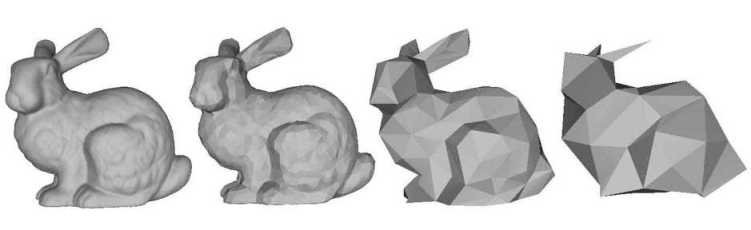
\includegraphics[width=0.8\columnwidth]{LODs-of-a-bunny-model-Courtesy-Stanford-3D-Scanning-Repository-From-left-to-right}
\caption{Level Of Detail Visualisierung vier Hasen \cite{stanfordBunnyModel}}
\label{fig:LevelOfDetailVisualisierungvierHasen}
\end{figure}

Wie in der Abbildung \ref{fig:LevelOfDetailVisualisierungvierHasen} zu erkennen ist, wird von links nach rechts der Detailgrad und somit die Komplexität des Objektes reduziert. Sind es im Bild ganz links noch 69'451 Polygone, wird es bereits im ersten Schritt auf 2'502 Polygone reduziert. Dies ist eine enorme Reduktion von ca. 96.5\%. Im dritten Schritt wird die Anzahl Polygone wiederum um ca. 90\% auf 251 reduziert. Schlussendlich hat das letzte Objekt noch 76 Polygone was knapp 0.1\% der ursprünglichen Anzahl entspricht.

\subsection{Ansätze für \e{LOD} Artefakte}
\label{chap:differentLodApproaches}
Es gibt verschiedene Ansätze, 3D-Modelle mittels \e{LOD} zu vereinfachen. In diesem Abschnitt werden einige davon detaillierter erläutert so wie ihre Vor- und Nachteile aufgezeigt.

\paragraph{Diskrete LOD (LDOD)}
Bei diskreten \e{LOD} werden für ein detailliertes Modell mehrere weniger detaillierte Modelle erstellt.
Abhängig von der Distanz zum Betrachter wird das optimale Modell gewählt. Es sind hierfür nur minimale Anpassungen am \fgls{Scene Graph}{Datenstruktur, welche die räumliche Anordnung der Modelle einer 3D-Szenerie beschreibt} notwendig da ausschliesslich ganze Modelle ausgetauscht werden.
Ein Nachteil sind jedoch merkbare harte Grenzen. Der Benutzer stellt beim umhergehen in der Szene fest, wenn das Modell mit einer einfacheren Version ausgetauscht wird.
Es ist zudem häufig nicht möglich grössere Modelle sinnvoll zu vereinfachen. Grosse Modelle zeichnen sich dadurch aus, dass Teile davon nah sind, während andere Teile fern sind. Die nahen Teile des Modells sollten detailliert angezeigt werden, wohingegen die entfernten Elemente vereinfacht dargestellt werden sollen. So ist der Ansatz zum Beispiel für Terrain ungeeignet. Ähnlicher Weise ist es auch nicht möglich, viele sehr kleine Modelle zu kombinieren, da jedes Modell unabhängig ist. Das Kombinieren von mehreren Modellen wird \e{Clustering} genannt.

\paragraph{Kontinuierliche LOD (CLOD)}
Im Gegensatz zu \e{DLOD} wird bei \e{CLOD} vereinfachende Veränderungen an einem Modell gespeichert.

Der Hauptunterschied zu \e{DLOD} besteht in den weichen Grenzen, so ist es signifikant weniger auffällig da zwischen den verschiedenen Auflösungen interpoliert werden kann.
Der Hauptnachteil ist jedoch, dass diese Interpolation insbesondere Auswirkungen auf die Laufzeit Performanz der Applikation hat.
Das Problem des \e{Clusterings} ist auch für diese Variante nicht gelöst.

\paragraph{Hierarchische LOD (HLOD)}
Bei \e{HLOD} werden mehrere Objekte in einen \e{Cluster} gruppiert. Diese \e{Cluster} können mithilfe des \e{\gls{Scene Graph}s} definiert werden.
Hierarchische Systeme erlauben es somit, zum Beispiel Terrains optimal abzubilden. So werden Ausschnitte, welche nahe beim Benutzer sind mit hoher Auflösung dargestellt während weiter entferntere Teile der Umgebung mit weniger Details ausgestattet sind.
Zudem ist es möglich viele kleinere Objekte bei entsprechenden Distanzen zu kombinieren.
Der Hauptnachteil liegt darin, dass hierfür signifikante Anpassungen am \e{\gls{Scene Graph}} notwendig sind und für den Entwickler ein spürbarer Unterschied entstehen kann.

\subsection{Vergleich Algorithmen}
\label{chap:lodAlgorithmComparison}

Das Ziel des Algorithmus ist es, eine gegebene geometrische Struktur mit möglichst wenig \e{Triangles} so genau wie möglich zu approximieren.
Diese Art von Problem ist in der Literatur unter anderem als \e{Surface Simplification}, polygonale Simplifizierung, geometrische Simplifizierung oder Mesh Reduzierung bekannt.
Im folgenden Abschnitt wird auf die Grundidee einiger Kategorien eingegangen, um einen groben Überblick zu verschaffen.
Für mehr Informationen zu weiteren Ansätzen, siehe \e{Quadric-Based Polygonal Surface Simplification} Sektion 2.4 \cite{quadridBasedSurfaceSimplification}.

\paragraph{Vertex Dezimierung}
Algorithmen dieser Kategorie entfernen jeweils einen Vertex und triangulieren das entstehende Loch neu.
Eine weitere Möglichkeit ist das \e{Vertex Clustering}, hierbei wird ein Modell in verschiedene Gitterzellen aufgeteilt. Die Punkte innerhalb einer Gitterzelle werden dann in einen einzigen Punkt zusammengelegt. Die visuelle Annäherung dieser Algorithmen bei drastischen Vereinfachungen stellt jedoch häufig ein Problem dar für polygonale Modelle. Sogenannte \e{Point Cloud} können mit solchen Algorithmen schnell vereinfacht werden.
\e{Point Clouds} sind Vertices im dreidimensionalen Raum ohne zugehörige \e{Triangle}, also ohne Fläche (in Abbildung \ref{fig:pointCloudTorus} exemplarisch zu sehen). Diese Daten können das Resultat eines 3D-Scanners sein.

\begin{figure}[H]
  \centering
  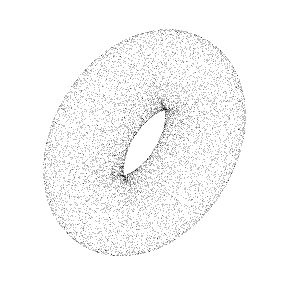
\includegraphics[width=0.4\columnwidth]{grundlagen/point-cloud-torus.png}
  \caption{Beispiel eines Torus visualisiert als \e{Point-Cloud} \cite{pointCloudTorus}}
  \label{fig:pointCloudTorus}
\end{figure}

\paragraph{Edge Collapse}
Hierbei werden iterativ \e{Edges} entfernt und die beiden \e{Vertices} zu einem Punkt zusammengelegt.
Die verschiedenen Algorithmen unterscheiden sich primär in der Selektion der \e{Edges}. Grundsätzlich wird hierfür eine Heuristik verwendet um den Fehler quantifizieren zu können. Anschliessend werden iterativ die \e{Edges} entfernt, welche zu einem minimalen Fehler führen. Beim Zusammenführen von \e{Edges} sind abhängig vom gewählten \e{LOD}-System unterschiedliche Strategien gefordert. Bei diskreten \e{LOD}-Systemen soll nach dem Zusammenführen ein optimaler neuer Punkt gefunden werden, bei kontinuierlichen \e{LOD}-Systemen wird häufig einer der beiden Punkte gewählt um Speicherplatz einsparen zu können.

\paragraph{Triangle Collapse}
Bei dieser Variante werden jeweils ganze Flächen entfernt und die umliegenden \e{Triangles} zusammengelegt. Eine Möglichkeit ist der von Hamann definierte Algorithmus zur Vereinfachung von triangulierten Flächen \cite{triangleCollapseAlgorithm}. Dabei wird die Krümmung eines \e{Triangles} definiert und iterativ derjenige \e{Triangle} mit der geringsten Krümmung entfernt. An die Stelle der drei \e{Vertices} tritt ein neuer \e{Vertex} und die umliegenden Flächen werden neu trianguliert.
